% -*- latex -*-
%%%%%%%%%%%%%%%%%%%%%%%%%%%%%%%%%%%%%%%%%%%%%%%%%%%%%%%%%%%%%%%%
%%%%%%%%%%%%%%%%%%%%%%%%%%%%%%%%%%%%%%%%%%%%%%%%%%%%%%%%%%%%%%%%
%%%%
%%%% This text file is part of the lecture slides for
%%%% `Parallel Computing'
%%%% by Victor Eijkhout, copyright 2012-2020
%%%%
%%%% Sharedmemory-slides.tex : slides about mpi shared memory
%%%%
%%%%%%%%%%%%%%%%%%%%%%%%%%%%%%%%%%%%%%%%%%%%%%%%%%%%%%%%%%%%%%%%
%%%%%%%%%%%%%%%%%%%%%%%%%%%%%%%%%%%%%%%%%%%%%%%%%%%%%%%%%%%%%%%%

\begin{numberedframe}{Shared memory myths}
  Myth:
  \begin{quote}
    MPI processes use network calls, whereas OpenMP threads access memory directly,
    therefore OpenMP is more efficient for shared memory.
  \end{quote}
  Truth:
  \begin{quote}
    MPI implementations use copy operations when possible, whereas OpenMP
    has thread overhead, and affinity/coherence problems.
  \end{quote}
  Main problem with MPI on shared memory: data duplication.
\end{numberedframe}

\begin{numberedframe}{MPI shared memory}
  \begin{itemize}
  \item Shared memory access: two processes can access each other's
    memory through \n{double*} (and such) pointers, if they are
    on the same shared memory.
  \item Limitation: only window memory.
  \item Non-use case: remote update. This has all the problems of
    traditional shared memory (race conditions, consistency).
  \item Good use case: every process needs access to large read-only
    dataset\\ Example: ray tracing.
  \end{itemize}
\end{numberedframe}

\begin{numberedframe}{Shared memory threatments in MPI}
  \begin{itemize}
  \item MPI uses optimizations for shared memory: copy instead of
    socket call
  \item One-sided offers `fake shared memory': yes, can access another
    process' data, but only through function calls.
  \item MPI-3 shared memory gives you a pointer to another process'
    memory,\\
    \emph{if that process is on the same shared memory}.
  \end{itemize}
\end{numberedframe}

\begin{numberedframe}{Shared memory per cluster node}
  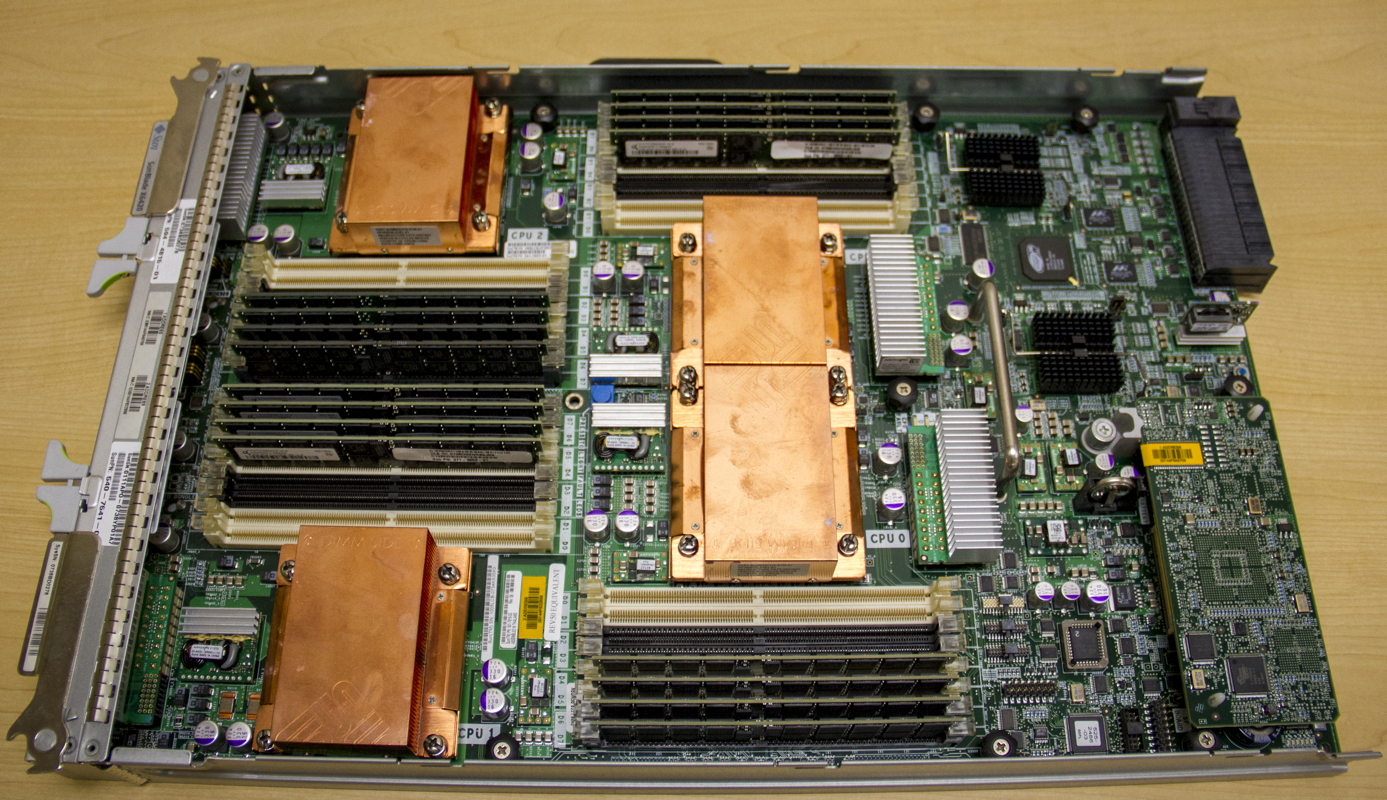
\includegraphics[scale=.45]{ranger-node-small}
  \begin{itemize}
  \item Cluster node has shared memory
  \item Memory is attached to specific socket
  \item beware \ac{NUMA} effects
  \end{itemize}
\end{numberedframe}

\begin{numberedframe}{Shared memory interface}
  Here is the high level overview; details next.
  \begin{itemize}
  \item Use \indexmpishow{MPI_Comm_split_type} to find processes on the same
    shared memory
  \item Use \indexmpishow{MPI_Win_allocate_shared} to create a window between
    processes on the same shared memory
  \item Use \indexmpishow{MPI_Win_shared_query} to get pointer to another
    process' window data.
  \item You can now use \n{memcpy} instead of \indexmpishow{MPI_Put}.
  \end{itemize}
\end{numberedframe}

\begin{numberedframe}{Discover shared memory}
  \begin{itemize}
  \item
    \indexmpishow{MPI_Comm_split_type} splits into communicators of same type.
  \item Use type: \indexmpishow{MPI_COMM_TYPE_SHARED} splitting by
    shared memory.\\
    (MPI-4: split by other hardware features through \indexmpishow{MPI_COMM_TYPE_HW_GUIDED}
    and \indexmpidef{MPI_Get_hw_resource_types})
  \end{itemize}

  { 
    \renewcommand\snippetcodefraction{.4}
    \renewcommand\snippetlistfraction{.55}
    \renewcommand\snippetoutputsize{\scriptsize}
    \csnippetwithoutput{commsplittype}{examples/mpi/c}{commsplittype}
    }
  %\cverbatimsnippet{commsplittype}
\end{numberedframe}


\begin{exerciseframe}
  \input{ex:mpi-node-proc-split}
\end{exerciseframe}

\begin{numberedframe}{Allocate shared window}
Use \indexmpishow{MPI_Win_allocate_shared} to create a window that can
be shared;
\begin{itemize}
\item Has to be on a communicator on shared memory
\item Example: window is one double.
\end{itemize}
\cverbatimsnippet[code/mpi/shared.c]{mpisharedwindow}
\end{numberedframe}

\begin{numberedframe}{Get pointer to other windows}
  Use \indexmpishow{MPI_Win_shared_query}:
  \cverbatimsnippet[code/mpi/shared.c]{mpisharedpointer}
\end{numberedframe}

\protoslide{MPI_Win_shared_query}

\begin{numberedframe}{Allocated memory}
  Memory will be allocated contiguously\\
  convenient for address arithmetic,\\ not for NUMA:
  set \indextermtt{alloc_shared_noncontig} true in
  \indexmpishow{MPI_Info} object.  

  Example: each window stores one double. Measure distance in bytes:
  \begin{multicols}{2}
    Strategy: default behavior of shared window allocation
\begin{verbatim}
Distance 1 to zero: 8
Distance 2 to zero: 16
\end{verbatim}
\columnbreak
Strategy: allow non-contiguous shared window allocation
\begin{verbatim}
Distance 1 to zero: 4096
Distance 2 to zero: 8192
\end{verbatim}
  \end{multicols}
Question: what is going on here?
\end{numberedframe}

\begin{numberedframe}{Exciting example: bulk data}
  \begin{itemize}
  \item Application: ray tracing:\\
    large read-only data strcture describing the scene
  \item traditional MPI would duplicate:\\
    excessive memory demands
  \item Better: allocate shared data on process~0 of the shared communicator
  \item Everyone else points to this object.
  \end{itemize}
\end{numberedframe}

\endinput

\begin{numberedframe}{}
\begin{lstlisting}
  
\end{lstlisting}
\end{numberedframe}

